\documentclass{beamer}
\usepackage{HECbeamer}
% \usepackage{pgfpages}
% \pgfpagesuselayout{4 on 1}[letterpaper, landscape, border shrink=5mm]
\title[\color{white}{MATH 60604A \S~5d - Compound symmetry model}]{\texorpdfstring{MATH 60604A \\Statistical modelling \\ \S~5d - Compound symmetry model}{MATH 60604A \\Statistical modelling \\ \S~5d - Compound symmetry model}}
\author{}
\institute{HEC Montréal\\
Department of Decision Sciences}
\date{} 

\begin{document}
\frame{\titlepage}


\begin{frame}
\frametitle{Covariance structure of the compound symmetry model}
\bi
\item Assume that the observations within a group are interchangeable. That is, 
assume that the correlation (conditional on the explanatory variables) between two $Y$ observations within a group is always the same, and that the conditional variance of $Y$ is constant.
\item In this case, if there are five observations within group $i$, the associated within-group covariance matrix is

{\small \[
\bs{\Sigma}_i=
  \begin{pmatrix}
    \sigma^2+\tau & \tau & \tau & \tau & \tau\\
    \tau & \sigma^2+\tau & \tau& \tau & \tau\\
    \tau & \tau & \sigma^2+\tau & \tau & \tau\\
    \tau & \tau & \tau & \sigma^2+\tau & \tau\\
    \tau & \tau & \tau & \tau & \sigma^2+\tau
  \end{pmatrix}.
\]
}
\item Note here is that the conditional covariance between two observations in the same group is $\tau$, and that the conditional variance of each observation is $\sigma^2+\tau$.
\ei
\end{frame}

\begin{frame}
\frametitle{Correlation structure of the compound symmetry model}
The corresponding correlation matrix for the compound symmetry covariance model is
\[
\mathbf{R}_i=
  \begin{pmatrix}
   1 & \rho & \rho & \rho & \rho\\
    \rho &1 & \rho & \rho & \rho\\
   \rho & \rho & 1 &\rho & \rho\\
   \rho & \rho & \rho & 1 &\rho\\
   \rho & \rho & \rho & \rho &1
  \end{pmatrix},
\]
where $\rho=\tau/(\sigma^2+\tau)$.
\bi
\item The conditional correlation between two observations within a group
is always $\rho$. 
\item This covariance structure is called ``\alert{compound symmetry}'' and has two parameters, $\sigma^2$ and $\tau$.
\ei
\end{frame}

 \begin{frame}[fragile]
\frametitle{\texttt{mixed} procedure to fit models to correlated data}
\begin{tcolorbox}[colback=white, colframe=hecblue, title=\SASlang{} code ]
\begin{verbatim}
/* Copy t */
data revenge; 
set statmod.revenge; 
tcat=t; 
run;

proc mixed data=revenge method=reml; 
class id tcat; 
model revenge = sex age vc wom t / solution; 
repeated tcat / subject=id type=cs r=1 rcorr=1; 
run;
\end{verbatim}
\end{tcolorbox}

\end{frame}
% 
% \begin{frame}[fragile]
%  \frametitle{Syntax for \code{proc mixed}}
%  \begin{center}
%  \includegraphics[width = 0.9\linewidth]{img/c5/06-correlated-proc_mixed_syntax.pdf}
%  \end{center}
% \end{frame}


 \begin{frame}[fragile]
\frametitle{Declaring the dependence structure within \code{proc mixed}}
The command \code{\textbf{repeated}} allows us to define the dependence structure.
\bi
\item The first argument of the \code{\textbf{repeated}} function specifies what order the observations are within each group. This variable must be a categorical variable (created via \code{\textbf{class}}). 
\item The option \code{\textbf{subject}} specifies the variable which identifies the groups. 
\item  The option \texttt{\textbf{type}} specifies the model for the within-group correlation.
\item The option \code{r=1} (\code{rcorr=1}) adds the estimated covariance (correlation) matrix for individual 1 in the output.
\ei 
{\footnotesize  We will also use the variable \code{t} as a continuous variable in the model, which is why we also created a copy of the variable \code{t} (\code{tcat} here), in order to use it as an argument for  \code{\textbf{repeated}}. 

}

\end{frame}
\begin{frame}[fragile]
\frametitle{Technical aside}
\bi
\item The first argument \texttt{tcat} in the \textbf{\code{repeated}} command is ignored here, as the compound symmetry covariance structure does not use the order of the observations within a group.
\item However, the order must be specified for other types of structures. It's good to specify the ``repeated" argument, even when it's not necessary.
\ei
\end{frame}

\begin{frame}[fragile]
\frametitle{Model specification}
\begin{center}
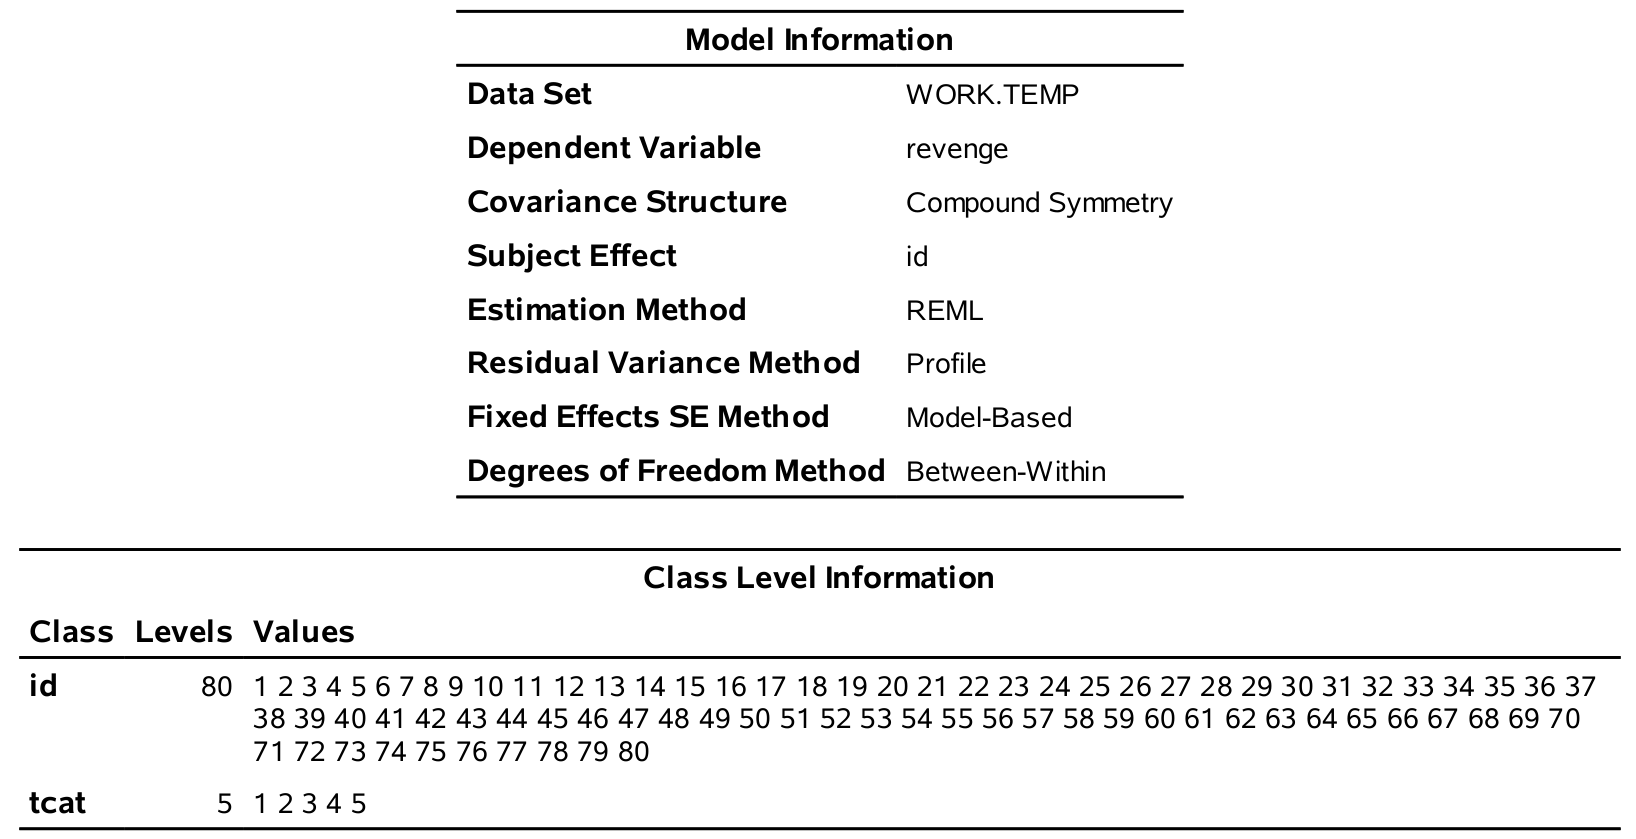
\includegraphics[width = \linewidth]{img/c5/slides6-e06}

\end{center}
% \bi
% \item In the upper-right hand table, $X$ represents the matrix of fixed effects and $Z$ the matrix of random effects. 
% \bi 
% \item There are no random effects in the model (more on this later).
% \ei
% \ei
\end{frame}

\begin{frame}[fragile]
\frametitle{Covariance and correlation matrices for individual $1$}
\begin{center}
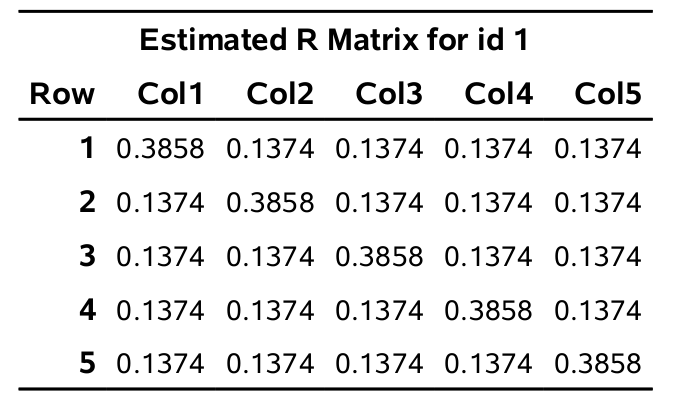
\includegraphics[width = 0.45\linewidth]{img/c5/slides6-e07a}
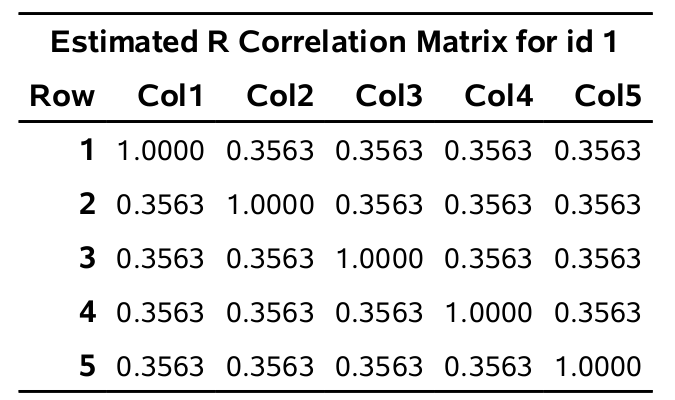
\includegraphics[width = 0.45\linewidth]{img/c5/slides6-e07b}
\end{center}
Since we specified a compound symmetry structure for the covariance, the correlation is the same for all observations within subject $1$.

\end{frame}

\begin{frame}[fragile]
\frametitle{Parameters for the covariance structure}
\begin{center}
% \includegraphics[scale=0.4]{Figures/long16_2b}
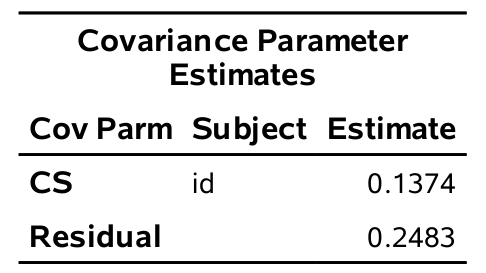
\includegraphics[width = 0.4\linewidth]{img/c5/slides6-e08}
%\includegraphics[scale=0.4]{Figures/long18.pdf}
\end{center}
\bi
\item The compound symmetry covariance structure is  
\bi
\item $\Va{Y_{ij}}=\sigma^2+\tau$;
\item $\Co{Y_{ij}, Y_{ij'}}=\tau$.
\ei
\item The estimate of the conditional covariance between observations for the same person is $\hat{\tau}=0.137$. 
\item The estimated conditional variance of an observation is $\hat{\tau}+ \hat{\sigma}^2= 0.386$.
\ei
\end{frame}

\begin{frame}[fragile]
\frametitle{Correlation structure}
\bi

\item The estimate of the conditional correlation between two observations from the same person (within-person correlation) is
\begin{align*}
\hat{\rho}=\frac{\hat{\tau}}{\hat{\tau}+\hat{\sigma}^2}=\frac{0.137}{0.137+0.248}=0.356.
\end{align*}
\item We can recover these values in the covariance/correlation matrices given for the first individual.
\item \textbf{You need to know how to retrieve the correlation based on output (hence the formulae.)}
\ei
\end{frame}
% \begin{frame}[fragile]
% \frametitle{Wald test for the covariance parameter}
% \begin{center}
% \includegraphics[scale=0.4]{Figures/long16_2b}
% %\includegraphics[scale=0.4]{Figures/long18.pdf}
% \end{center}
% \bi
%  \item Testing within-group correlation is equivalent to testing $\Hy_0: \tau=0$ against $\Hy_1: \tau \neq 0$.
% \item  The table ``\texttt{Covariance Parameter Estimates}'', reports the Wald test statistic $\hat{\rho}/\se(\hat{\rho})$  (\code{Z Value}).
% \item The asymptotic null distribution is standard normal, $\Cn(0,1)$.
% \item The $p$-value is negligible.
% \item According to the Wald test, there is a significant non-zero correlation between observations from the same person, even after accounting for the predictor variables. Moreover, this correlation is positive.
% \ei
% \end{frame}

\begin{frame}[fragile]
\frametitle{Likelihood ratio test for covariance parameter}

\begin{center}
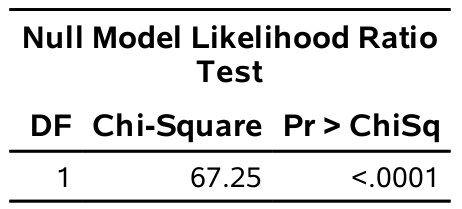
\includegraphics[width = 0.35\linewidth]{img/c5/slides6-e09}
\end{center}
\bi
\item 
We can  test $\Hy_0:\tau=0$ against $\Hy_1: \tau \neq 0$ using the \textbf{likelihood ratio test}.
\item The above table gives the likelihood ratio test for $\Hy_0: \tau=0$, which corresponds to the covariance model of the classic regression model with covariance $\sigma^2\mathbf{I}$ (reduced model), but ajusted using REML.
\item We conclude that the reduced model without a correlation structure is \textbf{not an adequate simplification} of the more complex model with the compound symmetry correlation structure. 
\item \textbf{The likelihood ratio test reported by \SASlang{}{} always perform the comparison with the homoscedastic linear model without correlation.}
\ei
% \item We can do the test manually: the linear model without any structure had $-2\ell_{\textrm{reml}}(\hat{\bs{\theta}}_0)=776.7.$
\end{frame}
\begin{frame}[fragile]
\frametitle{Likelihood ratio test, by hand}
\begin{center}
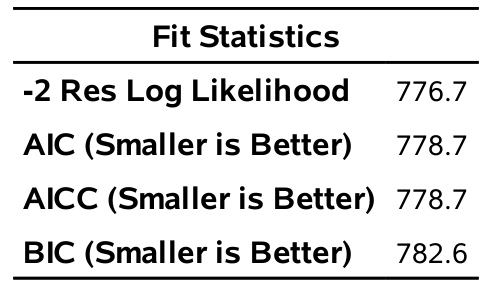
\includegraphics[width = 0.35\linewidth]{img/c5/slides6-e10}
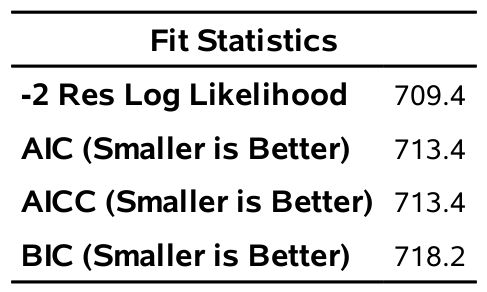
\includegraphics[width = 0.35\linewidth]{img/c5/slides6-e11}
\end{center}
\bi 
\item We could obtain the value of the test statistic manually by comparing the restricted maximum likelihood estimates of the two models, here $-2\ell_{\textrm{reml}}(\hat{\bs{\theta}}_0)=776.7$ and $-2\ell_{\textrm{reml}}(\hat{\bs{\theta}})=709.4$, so the likelihood ratio test statistic is $67.3$. 
\bi
\item {\footnotesize This is the value reported on the previous slide, modulo rounding. }
\ei 
\item The null distribution of the likelihood ratio test is $\chi^2_1$ (why?).
\item We can compare the value of the test to the $95\%$ quantile of the $\chi^2_1$, $3.84$. Since the value of the statistic is larger than $3.84$,  we reject $\Hy_0$ at level $\alpha=0.05$.
\ei
\end{frame}

\begin{frame}[fragile]
\frametitle{Mean parameter estimates}
\begin{center}
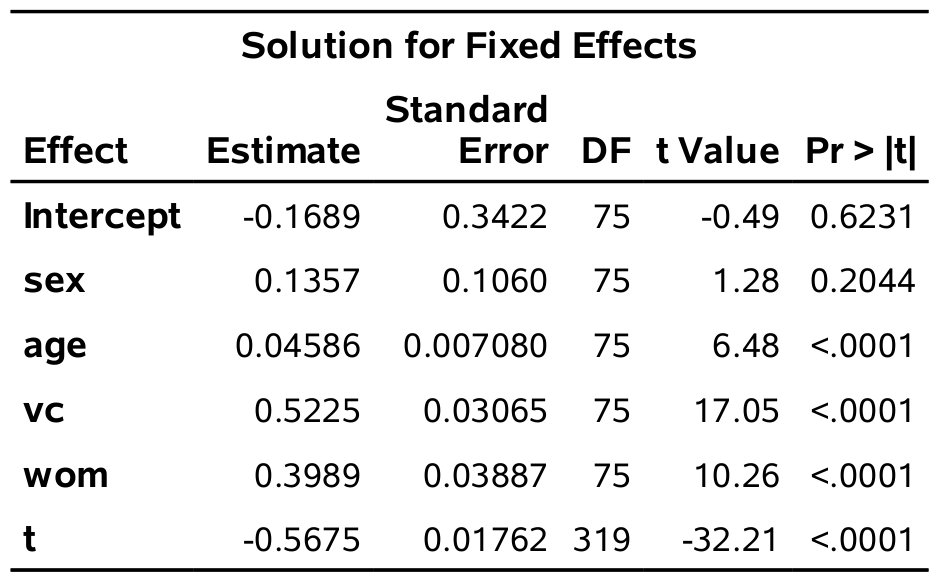
\includegraphics[width = 0.7\linewidth]{img/c5/slides6-e12}
\end{center}
Desire for revenge seems to decrease in time, after accounting for the other variables.
\end{frame}

\begin{frame}[fragile]
\frametitle{Coefficient estimates}
\bi
\item The fitted model is always a linear regression model,
\begin{align*}
\widehat{\code{revenge}}=&-0.169 + 0.136 \code{sex} + 0.0459 \code{age} + 0.523 \code{vc}\\
 & \qquad + 0.399 \code{wom} -0.568 \code{t}.
\end{align*}
\item  It turns out that the estimates $\hat{\bs{\beta}}$ are exactly the same as we saw in the ordinary linear regression model. 
\item This is a special case (compound symmetry correlation, and same number of observations in each group) and \alert{will not always be true for other models}. 
\item However, these estimates will usually be close to those coming from ordinary linear regression. 
\ei
\end{frame}




\begin{frame}[fragile]
\frametitle{Model comparison for coefficients}

\begin{center}
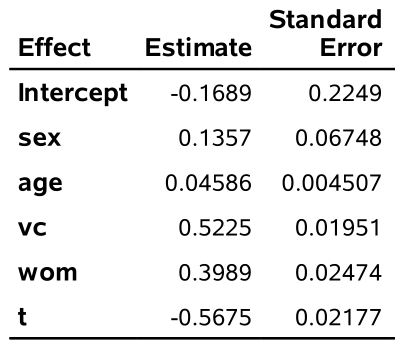
\includegraphics[width = 0.35\linewidth]{img/c5/slides6-e13}
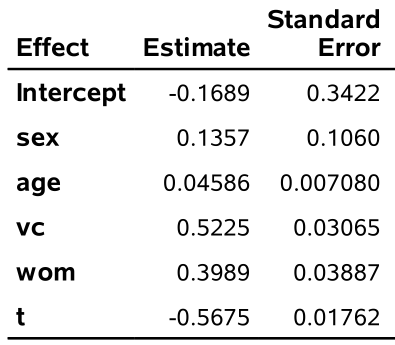
\includegraphics[width = 0.35\linewidth]{img/c5/slides6-e14}
\end{center}
\bi
\item The precision of our estimates $\hat{\bs{\beta}}$ changes (left is independence, right is equicorrelation model).
\item The standard errors are greater in the model with non-zero correlation. The conclusions did not change for any of the predictor variables, except for \code{sex}. It is no longer significant.
\item In fact, the correlations make within-person observations redundant to an extent. We actually have less information than we would for independent observations, so parameter estimates are less precise.

\ei
\end{frame}

\end{document}
